% flashcards-title: Thirty-five squares per hundred
% flashcards-desc: A ten by ten grid has thirty-five cells shaded.
\documentclass[dvisvgm,tikz,border=8pt]{standalone}\usetikzlibrary{arrows.meta,patterns}

\definecolor{qraNavy}{HTML}{17324D}
\definecolor{qraBlue}{HTML}{2B6CB0}
\definecolor{qraGold}{HTML}{B7791F}
\definecolor{qraPale}{HTML}{EAF2F8}
\definecolor{qraGray}{HTML}{5C6773}

\tikzset{
  qra axis/.style={draw=qraNavy, line width=1.2pt},
  qra tick/.style={draw=qraNavy, line width=1pt},
  qra guide/.style={draw=qraGray, densely dashed, line width=0.8pt},
  qra counter/.style={circle, draw=qraNavy, fill=qraPale, line width=0.9pt, minimum size=7mm, inner sep=0pt},
  qra label/.style={font=\sffamily\bfseries, text=qraNavy},
  qra small label/.style={font=\sffamily, text=qraNavy},
}

\begin{document}
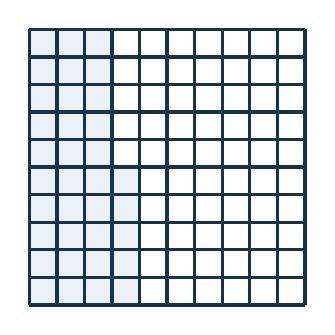
\begin{tikzpicture}[x=.35cm,y=.35cm]
  \foreach \n in {0,...,34}{
    \pgfmathtruncatemacro{\x}{floor(\n/10)}
    \pgfmathtruncatemacro{\y}{mod(\n,10)}
    \fill[qraPale] (\x,\y) rectangle (\x+1,\y+1);
  }
  \foreach \i in {0,...,10}{
    \draw[qra axis] (\i,0) -- (\i,10);
    \draw[qra axis] (0,\i) -- (10,\i);
  }
\end{tikzpicture}
\end{document}
